\chapter{Entropy bounds}
\label{chap:entropybound}

\section{Key rate}

To asses the performance of DIQKD protocols we need to compute the \textit{key rate}, labelled $r$, corresponding to the amount of key bit that can be extracted per round.
We here solely focus on asymptotic key rates, which are key rates derived in the limit of an infinite number of rounds.
If asymptotic key rates are fundamentally inaccessible, they are a handy tool to asses the quality of a DIQKD protocol.
In particular, avoiding finite size effects greatly simplify the computation of key rates.
However, by not including these finite size effects, the asymptotic regime yield key rates higher that the ones obtained for a finite number of rounds.
These finite size effects are beyond the scope of this thesis, some details can be found in ~\cite{Tan2021,Tan2022,Primaatmaja2023}.

Extracted key bits must be secret, i.e. provably unknown to Eve, and correct, i.e. identical for Alice and Bob.
Therefore, the computation of a key rate must take into account all attacks that can be implemented by Eve, and specific error-correction protocol.
In the following, we discuss key rates that were first derived with the assumption that quantum devices are independent and identically distributed (IID) over the rounds of the protocols, i.e. that the devices are memoryless, measurements $\hat{A}_x,\hat{B}_y$ are the same through the protocol and the distributed state for $n$-round is of the form $\ket{\psi}_{ABE}^{\otimes n}$.
This assumption limits Eve's range of attack to what is known as collective attack.
However, using the \textit{entropy accumulation theorem}~\cite{Dupuis2019,Dupuis2020}, it has been shown that the key rates we present here, up to some finite corrections, hold under general attacks, known as coherent attacks, allowing to drop the need for the IID assumption~\cite{ArnonFriedman2019}.
Note that in the asymptotic regime, there exists a choice of protocol parameters that render the cost of these the finite corrections negligible.


\medbreak

Intuitively, the key rate is given by the mutual information between the outcomes of the generation rounds, $A_0$ and $B_2$, used to generate the key (correctness) and is limited by the amount of information Eve has on $A_0$ (secrecy).
In the asymptotic limit, where one-way error correction from Alice to Bob is used and where the correlations $p(ab|xy)$ can be computed exactly, the key rate is lower-bounded by the Devetak-Winter bound~\cite{Devetak2005}
\begin{equation}
	r \geq r_\mathrm{DW} = I(A_0 : B_2) - \chi(A_0 : E)
	\label{eq:Devetak-Winter}
\end{equation}
where $I$ is the mutual information, $\chi$ corresponds to the Holevo bound and $E$ denotes the quantum-side information Eve stored during the protocol.
Note that the key rate can be expressed using conditional von Neumann entropies $H(\centerdot|\centerdot)$ following
\begin{equation}
	\begin{split}
		r_\mathrm{DW} &= I(A_0 : B_2) - \chi(A_0 : E) \\
					  &= H(A_0)-H(A_0|B_2) - (H(A_0)- H(A_0|E)) \\
					  &= H(A_0|E) - H(A_0 | B_2).
	\end{split}
\end{equation}

The remaining challenge is to bound these two term, and in particular to upper-bound the Holevo quantity directly from the correlations $p(ab|xy)$, as no assumption can be made on Eve's system and the quantum devices. 
In the following two sections we will described two methods to tackle this bound, the first one utilizing the CHSH score, the second one is based on a more refined analysis of the correlations.

\section{CHSH-based security}

\subsection{Key rate from the CHSH score}
\label{sec:pironio}

In \cite{Pironio2009}, the first upper-bound on the Devetak-Winter bound has been derived.
This approach makes use of an additional symmetrisation step in the protocol presented in the previous chapter.
The symmetrisation step allow Alice and Bob to obtain uniform marginals, which result in $H(A_x)=H(B_y)=1$.
In order to do so, Alice and Bob can simply XOR their key bits with a public random string that is shared over the classical channel.

Let's consider uniform noise, i.e. noise affecting symmetrically the outcomes of Alice and Bob's measurements.
Such type of noise naturally occurs when a state goes through a depolarizing channel or through a phase-covariant cloner.
In that case, the mutual information between Alice and Bob's raw key simply reads
\begin{equation}
	I(A_0 : B_2) = H(A_0) - H(A_0|B_2) = 1 - h(Q)
\end{equation}
where $Q=p(a=b|xy)-p(a\neq b |xy)$ is the quantum error bit rate (Qber) and $h$ is the binary entropy $h(x)=-x \log_2(x) - (1-x)log_2(1-x)$.

From the parameter estimation step of the protocol presented above, Bob can compute the CHSH score $S=\mean{\hat{A}_0 \hat{B}_0} + \mean{\hat{A}_0 \hat{B}_1} + \mean{\hat{A}_1 \hat{B}_0} - \mean{\hat{A}_1 \hat{B}_1}$.
From this score and using Jordan's lemma, an upper-bound on the Holevo quantity appearing in \refeq{Devetak-Winter} is derived
\begin{equation}
	\chi(A_0 : E) \leq h\left(\frac{1+\sqrt{(S/2)^2-1}}{2} \right).
	\label{eq:holevo_pironio}
\end{equation}

Finally, from this two results, a lower bound on the DIQKD key rate is given by
\begin{equation}
	r \geq r_\mathrm{P} = 1 - h\left(\frac{1+\sqrt{(S/2)^2-1}}{2} \right) - h(Q).
	\label{eq:pironio}
\end{equation}

\subsection{Fine-grained error-correction}
\label{sec:Ma_Lutk}

When presenting the protocol in the previous chapter, we assumed that Alice and Bob have binary measurements with outcomes $\pm 1$.
A more general approach would allow both parties to have measurements with more outcomes, that could ultimately be binned to form the raw key.
Non-binary outcomes naturally occur in the presence of loss, as loss might lead to no measurement outcomes, which can be accounted as an extra outcome.
Interstingly, Bob can use the extra information of the non-binned or \textit{fine} outcomes of $B_2$ to reduce the cost of error-correction~\cite{Ma2012}.
This \textit{fine-grained error correction} is given by
\begin{equation}
	\begin{split}
		I(A_0 : B_2) &= 1-H(A_0|B_2) \\
					 &= 1-H(A_0,B_2) - H(B_2) \\
					 &= 1-\sum_b \left( \sum_{a = \pm1} -p(ab|02)\log_2(p(ab|02)) \right) \\
					 &\qquad - p(b|02)\log_2(p(b|02)).
	\end{split}
	\label{eq:Ma}
\end{equation}
Note that, in the case of uniform noise, this error-correction trivially reduces to $1-h(Q)$ in case Bob has only two outcomes.

Therefore, a tighter lower-bound on the key rate is
\begin{equation}
	r \geq r_\mathrm{ML} = 1 - h\left(\frac{1+\sqrt{(S/2)^2-1}}{2} \right) - H(A_0|B_2).
	\label{eq:Makr}
\end{equation}


\subsection{Noisy Preprocessing}

In the case of device-dependent QKD~\cite{Renner2005,Kraus2005,Renes2007}, it has been shown that Eve's uncertainty might increase if Alice includes a \textit{noisy-preprocessing} step following the measurement step of the DIQKD protocol we consider here~\cite{Ho2020}.
This noise acts as a bit-flip operation on the binned outcome of $\hat{A}_0$, used for key generation, occurring with a probability $q$, fixed by Alice.
Formally, this is the transformation
\begin{equation}
	p(a|0y) \rightarrow (1-q)\,p(a|0y) + q\, p(-a|0y).
\end{equation}
We denote $A_0'$ the raw key bit of Alice after noisy pre-processing.

For a CHSH score $S$ and a noisy preprocessing probabliy $q$, the Holevo quantity is upper bounded by
\begin{equation}
	\begin{split}
		\chi(A_0' : E) \leq I_q(S) = &h\left(\frac{1+\sqrt{(S/2)^2-1}}{2}\right) \\
									&-h\left(\frac{1+\sqrt{1-q(q-1)(8-S^2)}}{2} \right),
	\end{split}	
\end{equation}
which is equivalent to \refeq{holevo_pironio} when $q=0$, and smaller otherwise.

Combined with the fine-grained error-correction term \refeq{Ma}, we obtain the following lower bound on the key rate
\begin{equation}
	r \geq r_\mathrm{Ho} = 1 - I_p(S) - H(A_0'|B_2).
	\label{eq:Ho}
\end{equation}


\subsection{Robustness of CHSH-based security}
\label{sec:robust_DIQKD}

To grasp the requirements for experimental implementations of DIQKD, we need to study the behaviour of the key rate for some specific quantum model and losses.

\medbreak

Intuitively, it is worth exploring the behaviour of the key rate when the source sends a singlet state $\ket{\psi}=\frac{1}{\sqrt{2}}(\ket{00}+\ket{11})$, as this state saturate the CHSH inequality and thus should yield a key rate of $1$ in the absence of losses.

We consider measurements to be as general as possible on the $(\sigma_x-\sigma_z)$-plane. This is, measurements characterized by the POVMs associated with outcomes $\{+1,-1\}$
\begin{equation}
	\begin{split}
		\hat{A}_x\,:\, \{M(\alpha_x),\, \id-M(\alpha_x)\} \\
		\hat{B}_y\,:\, \{M(\beta_y),\, \id-M(\beta_y)\}
	\end{split}	
\end{equation}
with $M(\theta) = \frac{1}{2}\left(\id + \cos(\theta)\sigma_z + \sin(\theta)\sigma_x \right)$ and the angles $\alpha_x,\beta_y\in[0,\pi/2]$.
To verify our intuition in the absence of loss, without noisy preprocessing $q=0$, and with the optimal angles $(\alpha_0,\alpha_1)=(0,\pi/2)$ and $(\beta_0,\beta_1,\beta_2)=(\pi/4,-\pi/4,0)$, we indeed obtain a key rate of
\begin{equation}
	r \geq 1-h\left(\frac{1+\sqrt{(S/2)^2-1}}{2}\right)-h(Q) = 1 - h(1) - h(1) = 1.
\end{equation}

In the presence of loss, we need to address the possibility of the shared state being lost before the measurement, which would result in the absence of outcome.
We label $\eta\in[0,1]$ the efficiency of the quantum devices, i.e. the shared state is lost with probability $1-\eta$.
If the state is lost, Alice and Bob can recover binary outcomes by binning the no-outcome event as $+1$.
Thus, their POVMs becomes
\begin{equation}
	\{M^{+1},\,M^{-1}\} \rightarrow \{\eta M^{+1}+(1-\eta) \id,\, 1-\left(\eta M^{+1}+(1-\eta) \id\right)\}.
\end{equation}
However for his measurement $B_2$, Bob can simply consider all three outcomes, with the corresponding POVM
\begin{equation}
	B_2\, : \, \{\eta M(\beta_2),\, \eta (1-M(\beta_2)),\, (1-\eta) \id \},
\end{equation}
since exploiting fine-grained outcomes can reduce the cost of error-correction as explained in Sec.~\ref{sec:Ma_Lutk}.

To study the robustness of CHSH-based key rates, we optimise the different key rates \refeq{pironio}, \refeq{Makr} and \refeq{Ho}, over all measurement angles $\alpha_x,\beta_y$ on the singlet state, for a decreasing efficiency $\eta$. 
When considering noisy preprocessing, we also optimize the key rate over the parameter $q$ of \refeq{Ho}.
These key rates are shown in figure \reffig{kr_singlet}. 
Most interestingly, using noisy preprocessing and fine-grained error-correction, we obtain a critical efficiency of $\eta \approx 0.903$, below which no key can be extracted.

For a more general approach, we study the robustness of the CHSH-based key rates for all partially entangled pure two-qubit states of the form
\begin{equation}
	\ket{\psi}_\theta = \frac{1}{2}\left(\cos(\theta)\ket{00}+\sin(\theta)\ket{11}\right)
	\label{eq:partiallyentangled}
\end{equation}
with $\theta\in[0,\pi]$.
This is done by adding the parameter $\theta$ as an optimisation parameters when optimising for the key rate.
The results are given in \reffig{kr_qubit}.
As expected from ~\cite{Eberhard1993}, the key rate is more tolerant to loss for these states, and the critical detection efficiency drop to $\eta\approx 0.826$.

\begin{figure}
     \centering
     \begin{subfigure}[b]{0.72\textwidth}
         \centering
         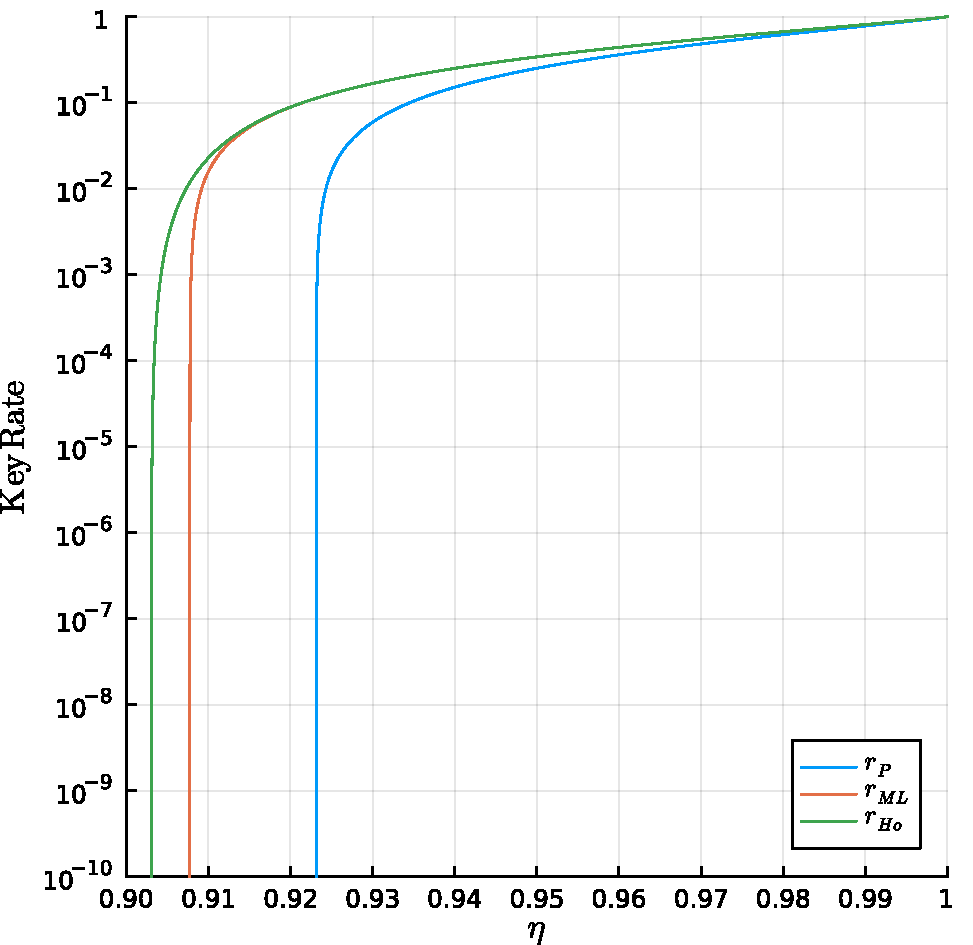
\includegraphics[width=\textwidth]{chapters/deviceindependent/img/key_rate_singlet.pdf}
         \caption{Two-qubit maximally entangled state}
         \label{fig:kr_singlet}
     \end{subfigure}
     \begin{subfigure}[b]{0.72\textwidth}
         \centering
         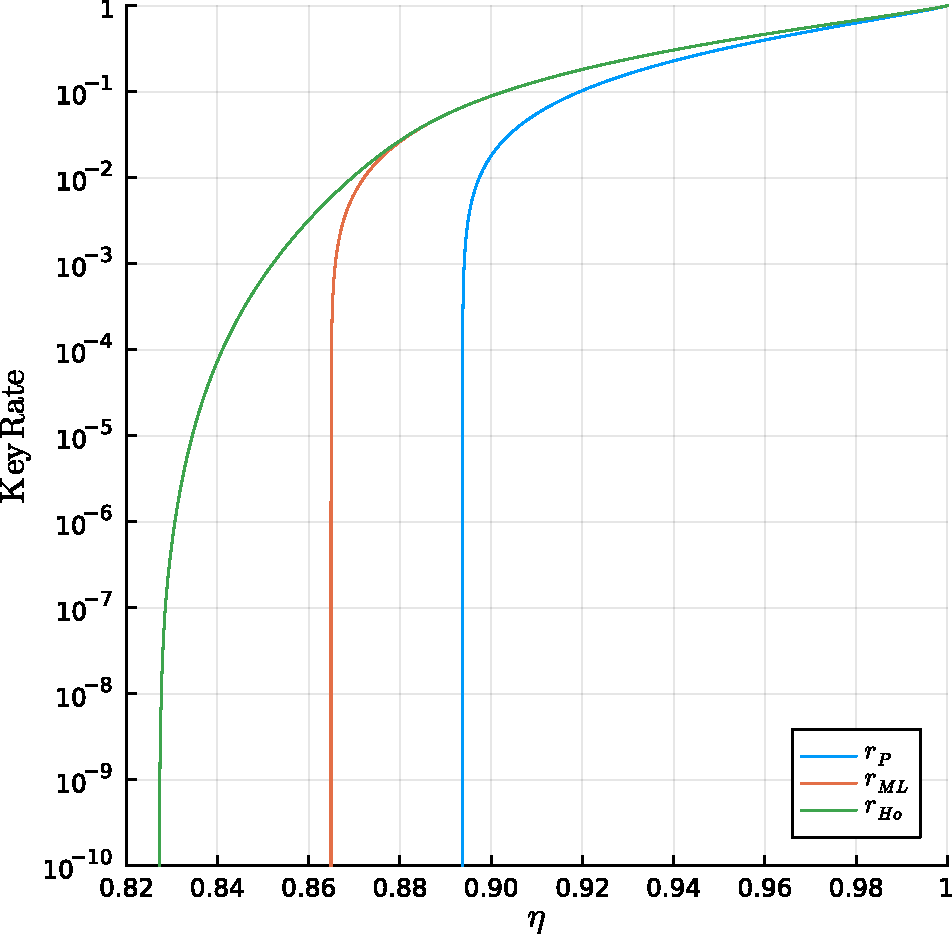
\includegraphics[width=\textwidth]{chapters/deviceindependent/img/key_rate_qubit.pdf}
         \caption{Two-qubit partially entangled state}
         \label{fig:kr_qubit}
     \end{subfigure}
	 \caption{Evolution of different key rates with efficiency $\eta$. $r_P$ is given by \refeq{pironio}, $r_{ML}$ by \refeq{Makr} and $r_{Ho}$ by \refeq{Ho}. The key rates are optimised over Alice and Bob measurement angles, and for insert b) over the parameter $\theta$ of \refeq{partiallyentangled}. }
 \end{figure}

\section{DIQKD security proof beyond CHSH}

In the previous section, we presented how provably secure key bits can be extracted from the CHSH score.
If improvement on the key rate has been made by including fine-grained error-correction and noisy preprocessing, the security proof is still fundamentally limited by the CHSH score.
To improve the resistance to losses, a natural approach is to derive a security statement from a more refined analysis of the observed statistics $\{p(ab|xy)\}$.
Conveniently, since the CHSH score is computed from these correlations, no extra step or assumption on the DIQKD protocol are required. 

\subsection{Security statement from the generalized-CHSH score}
\label{sec:Pavel}

The generalized CHSH score $S_\theta=\sqrt{2}(\cos(\theta)X+\sin(\theta)Y)$, obtained from the genrealized CHSH operator $\mathcal{B}_\theta$, allows to exploit the knowledge of the correlator pair
\begin{equation}
	\begin{split}
		X = \mean{A_0 \otimes (B_0+B_1)},\\
		Y = \mean{A_1 \otimes (B_0-B_1)}.
	\end{split}
\end{equation}
We have seen in the previous part that generalized CHSH inequalities, compared to CHSH, can be advantageous for a device-independent protocol that is self-testing~\cite{Valcarce2022}.
Intuitively, these inequalities can be useful for DIQKD as well.
The intuition comes from the correlator pair $X,Y$ allowing to differentiate between the contributions of measurements $\hat{A}_0$, used for key generation, and $\hat{A}_1$ solely used to test the quantum devices.
Therfore, this extra degree of freedom could allow us to bound Eve's entropy on the outcome $A_0$ more tightly.

In Article 3, we investigate this intuition, paving the way for DIQKD security proofs beyond the CHSH score. 
We here provide a sketch of the proof, for more detail please refer to \cite{Sekatski2021} or, alternatively, to \cite{Woodhead2021}.


\medbreak

%Binning the outcomes $A_x,B_y$ for $x,y\in\{0,1\}$, allow to utilize Jordan's lemma to express Alice and Bob observables as block diagonal operators on qubits
%\begin{equation}
%	\begin{split}
%		\hat{A}_x = \bigoplus_i \hat{A}_x^i &= \bigoplus_i \mathbf{\alpha_x^i} \begin{pmatrix}\sigma_z \\ \sigma_x\end{pmatrix}, \\
%		\hat{B}_y = \bigoplus_j \hat{B}_y^j &= \bigoplus_j \mathbf{\beta_y^i} \begin{pmatrix}\sigma_z \\ \sigma_x\end{pmatrix},
%	\end{split}
%\end{equation}
%with unit vectors $\mathbf{\alpha_x^i} = (\alpha_x^{i,0},\alpha_x^{i,1})$ and $\mathbf{\beta_y^j} = (\beta_y^{j,0},\beta_y^{j,1})$.
%Without loss of generality we can also write the shared state as
%\begin{equation}
%	\ket{\psi}_{ABE} = \bigoplus_{i,j} \sqrt{p_{i,j}} \ket{\psi}_{ABE}^{i,j}	
%\end{equation}
%with $\ket{\psi}_{ABE}^{i,j} \in \mathds{C}^2_A \otimes \mathds{C}^2_B \otimes \Hil_E^{(4)}$ and for some probability distribution $p_{i,j}$.
%This allow to express Eve's uncertainty on the key, after noisy preprocessing, as the convex sum
%\begin{equation}
%	H(A_0'| E) = \sum_{i,j} p_{i,j} H_{i,j}(A_0' | E)
%	\label{eq:H_convex}
%\end{equation}
%where $H_{ij}(A_0' | E)$ is computed from the state $\ket{\psi}_{ABE}^{i,j}$.
%To lower bound that quantity, we can minimize the entropy $H_{ij}(A_0 | E)$ over all four-qubits quantum model compatible with a generalized CHSH score $S_\theta$.
%If the minimization gives a convex function of $S_\theta$, from \refeq{H_convex}, that function acts as a lower bound on Eve's entropy. 
%If that is not the case, an extra convexification step can be added before obtaining the lower bound~\cite{Sekatski2021}.
%
%To simplify the minimization problem, we include a symmetrisation step, as explained in Sec~\ref{sec:pironio}, such that Alice and Bob have uniform marginals.
%Since no such marginals appear in the constraint of the minimization problem, the symmetrisation step allow to consider a minimization over only Bell diagonal states~\cite{Pironio2009}
%\begin{equation}
%	\ket{\psi}_{ABE}^{i,j} = \sum_k \sqrt{L_k^{i,j}} \ket{\phi_k} \otimes \ket{i}_E
%	\label{eq:psi_ABE_reduced}
%\end{equation}
%where $\ket{\phi_k}=\{\ket{\phi^+},\ket{\phi^-},\ket{\psi^+},\ket{\psi^-}\}$ are the Bell states defined in \refeq{bell_states} and $L_k$ are  eigenvalues we collect in a vector $\mathbf{L}=(L_1,L_2,L_3,L_4)$.
%
%The objective of the minimization, Eve's entropy, reads
%\begin{equation}
%	H(A_0'|E)_{i,j} = H(A_0') - H_{i,j}(\rho_E) + \sum_{a' = \pm 1} p(a'|x=0)H_{i,j}(\rho_{E|a'})	
%\end{equation}
%where $\rho_E$ is Eve's subsystem and $\rho_{E|a'}$ is Eve's subsystem conditioned on the key bit $a' = (1-q)\,a + q\,(-a)$ occurring with probability $p(a')$, for a noisy preprocessing bit flip probability of $q$.
%This expression can be simplified as $H(A_0')=1$ from the symmetrisation step.
%Furthermore, we have $H_{i,j}(\rho_E)=H_{i,j}(\mathbf{L})$ and $H_{i,j}(\rho_{E|a'})$ can be express as a function $f_{i,j}(\mathbf{L},\alpha_0^i)$ of the eigenvalues $\mathbf{L}$ and Alice's measurement angle $\mathbf{\alpha_0^i}$.

The critical part of the security analysis consists in bounding Eve's information on the key directly from the correlator pair $X,Y$.
This requires to analyze the entropy $H(A_0'|E)$ of Eve on the key $A_0'$ obtained after a noisy preprocessing with probability $q$, in a more refined way compared to the \acrshort{chsh} case.
This entropy can be expressed as 
\begin{equation}
	H(A_0'|E) = H(A_0') - \underbrace{\left(H(\rho_E) - \sum_{a'=\pm1}p(a')H(\rho_{E|a'})\right)}_{I_{\theta,q}(X,Y)}
\end{equation}
where $\rho_E$ is the reduced state of Eve, and where $\rho_{E|a'}$ is Eve's state conditioned on the key bit $A_0'=a'$, occuring with probability $p(a')$.
Using the symmetrisation step explained in Sec~\ref{sec:pironio}, we have $H(A_0')=1$.
We show in \cite{Sekatski2021} that, using Jordan's lemma, the quantity $I_{\theta,q}(X,Y)$ reduced on two-qubit states $I'_{\theta,q}(X,Y)$ can be obtained by solving the maximization problem
\begin{equation}
	\begin{split}
		I'_{\theta,q}(X,Y) = \max_{L,\alpha_0,\alpha_1,\beta_0,\beta_1} & H(\mathbf{L}) + H(\rho_{E|a'=+1}(L,\alpha_0,q)) \\
		&\mathrm{s.t.}\quad 
		\mathcal{B}_\theta (\mathbf{L},\alpha_0^i,\alpha_1^i,\beta_0^j,\beta_1^j) \geq S_\theta,
	\end{split}
\end{equation}
where $\rho_{E|a'=+1}(\mathbf{L},\alpha_0,q)$ is a two-qubit states shared between Alice and Eve, with a fixed dependency in $\alpha_0,\mathbf{L}$ and $q$, and where $\mathcal{B}_\theta (\mathbf{L},\alpha_0,\alpha_1,\beta_0,\beta_1)$ is the generalized CHSH operator parametrized by $\theta$ and Alice and Bob's measurement angles $(\alpha_0,\alpha_1,\beta_0,\beta_1)$ applied on states of the form
\begin{equation}
	\ket{\psi}_{AB} = \sum_k \sqrt{L_k} \ket{\phi_k},
	\label{eq:}
\end{equation}
with $\ket{\phi_k}=\{\ket{\phi^+},\ket{\phi^-},\ket{\psi^+},\ket{\psi^-}\}$, characterized by $\mathbf{L}=(L_1,L_2,L_3,L_4)$.
In \cite{Sekatski2021} we further explain how to solve this optimisation, and how to obtain the function $\tilde{I}_{\theta,q}(X,Y)\geq I'_{\theta,q}(X,Y)$ concave in $S_\theta$.

In Article 3, we solve the minimization for all $\theta\in[0,pi/2]$. This gave us the bound on the conditional entropy $1-\min_{\theta}\tilde{I}_{\theta,q}(X,Y)\leq H(A_0|E)$ and, hence, the lower bound on the key rate
\begin{equation}
	r \geq r_\mathrm{Sek} = 1 - \min_{\theta} \tilde{I}_{\theta,q}(X,Y) - H(A_0'|B_2).
	\label{eq:Sekatstki}
\end{equation}
Interestingly, this approach achieves higher key rate than CHSH-based key rates, except when correlators satisfies $X(X+Y)=4$ for which obtained key rates are equal.
When considering optimal noisy preprocessing, the gap in improved key rate diminish but is still non-neglectible.
Applied to the concrete case of a singlet state as explained in \ref{sec:robust_DIQKD}, the criticial detection efficiency drops from $\approx 0.903$ to $\approx 0.900$ when using generalized CHSH security proof.
However, for partially entangled two-qubit states, there is no improvement in critical detection efficiency.
Note that, independently to our results, \cite{Woodhead2021} reported on similar results. In particular, a DIQKD security proof has also been dervied from the generalized CHSH score and the reported advantages in key rate and critical efficiencies are indentical to the ones found using our method.

\medbreak


\subsection{Security statement from all correlations}
\label{sec:Brown}

In \cite{Brown2021} a device-independent lower bound on the von Neumann entropy has been derived based on all the correlations $\{p(ab|xy)\}$.
This approach introduces a sequence of optimisation problems which ultimately converges to the conditional von Neumann entropy, for states which lay in tensor product Hilbert spaces.
Each optimisation problem can be solved using a NPA hierarchy~\cite{Navascues2007,Pironio2010}, allowing to obtained a certified bound from semi-definite programming, and tightly converging with the order of the hierarchy.
As this method is more general than the scope of this thesis, we here briefly introduce the optimisation problem and the result of this method when applied to DIQKD key rate.

\medbreak

Consider a state $\rho_{ABE} \in \mathcal{\Hil_A} \otimes \mathcal{\Hil_A} \otimes \mathcal{\Hil_E} $ shared between Alice, Bob and Eve. 
The shared state reduced on Alice and Eve subsystems is given by $\rho_{AE}=\tr_B[\rho_{ABE}]$.
We label $\{M_a^0\}$ the POVM corresponding to the outcomes $\{a\}$ for Alice's measurement $\hat{A}_0$.
For some $m\in\mathds{N}$, lemma 3.1 of \cite{Brown2021} states that Eve's entropy on Alice's raw key is lower bounded by
\begin{equation}
	\begin{split}
		c_m + &\sum_{i=1}^{m-1}\frac{w_i}{t_i\ln(2)}\sum_a \inf_{Z_a\in \mathcal{L}(\Hil_E)} \tr\big[\rho_{AE} \\
			  &\qquad\left(M_a^0 \otimes (Z_a + Z_a^* + (1-t_i)Z_aZ_a^*+t_i(\id_A\otimes Z_a Z_a^*)\right)\big] \\
			  &\text{s.t.} \quad ||Z_a|| \leq \nu_i = \frac{3}{2}\max\left\{\frac{1}{t_i},\frac{1}{1-t_i}\right\}
	\end{split}
	\label{eq:Brown}
\end{equation}
where $c_m=\frac{-1}{m^2 \ln(2)}+\sum_{i=1}^m \frac{w_i}{t_i \ln(2)}$ and where $w_i$ and $t_i$ are the nodes and weights of the $m$-order Gauss-Radau quadrature in the range $[0,1]$.
\refeq{Brown} converges to $H(A_0|E)$ when $m$ converges to infinity.

To obtain a device-independent lower bound on the conditional von Neumann entropy, we can constraint \refeq{Brown} to  all quantum model compatible with the observed correlations. 
In particular, we define $r$ constraints as inequalities of linear combinations of the observed correlations 
\begin{equation}
	\sum_{abxy}c^i_{abxy}p(ab|xy) \geq \gamma_i \quad \forall i\in\{1,...,r\}.
\end{equation}
Adding these constraints and relaxing \refeq{Brown} by commuting the sum and the infinimum as well as by replacing the tensor product structure of the space of $\rho_{AE}$ by intrdoucing commutation relations on the relevant variables, one obtains the problem 
\begin{equation}
	\begin{aligned}
		c_m + \inf \sum_{i=1}^{m-1}\frac{w_i}{t_i\ln(2)}\sum_a 	\bra{\psi} M_a^0(Z_{a,i}+ Z_{a,i}^* +(1-t_i)Z_{a,i}Z_{a,i}^*+t_i(\id_A\otimes Z_{a,i} Z_{a,i}^*)\ket{\psi} \\
	\begin{alignedat}{3}
			  &\text{s.t.}\quad && \sum_{abxy} c^i_{abxy}\bra{\psi} M_a^x N_b^y \ket{\psi} \geq \gamma_i  &&\forall i\in\{1\,\dots,r\} \\
			  & && \sum_a M_a^x = \sum_b N_b^y = \id &&\forall x,y\\
			  & && M_a^x \geq 0 && \forall a,x\\
			  & && N_b^y \geq 0 && \forall b,y\\
			  & && Z_{a,i}Z_{a,i}^* \leq \nu_i &&\forall a, \; i\in\{1,\dots,m-1\} \\
			  & && Z_{a,i}^*Z_{a,i} \leq \nu_i &&\forall a, \; i\in\{1,\dots,m-1\} \\
			  & && [M_a^x,N_b^y]=[M_a^x,Z_{b,i}]=[N_b^y,Z_{a,i}] = 0 \qquad&&\forall a,b,x,y,i
	\end{alignedat}
	\end{aligned}
	\label{eq:NPA_DIQKD}
\end{equation}
where the minimum is taken over all collections $(\ket{\psi},\{M_a^x\},\{N_B^y\},\{Z_{a,i}\})$.
Using the NPA hierarchy, this problem can be relaxed into a converging sequence of semi-definite program, which can be solved exactly.

\medbreak

This method, when applied to correlations compatible with a two-qubit partially entangled state shared between Alice and Bob, gives the most advantageous key rate. 
We find that the critical detection efficiency, in particular, drops to $\approx 0.805$, considering a $(m=8)$-order Gauss-Radau quadrature.
This critical detection efficiency for two-qubit partially entangled states is real close to the optimal one, as it has been proven that no key rate can be obtain from efficiency below $\approx 0.7904$\cite{Lukanowski2022}.

Note, however, that this method requires heavy computational resources.
It is, henceforth, not convenient for a quick benchmark of a DIQKD implementation proposal.
In this scope, solving ~\refeq{NPA_DIQKD} more efficiently is desired, this could be achieve by choosing better monomial sets or by exploiting symmetries to reduce the size of the SDPs~\cite{Rosset2021}.
